\documentclass[border=10pt]{standalone}
\usepackage{pgfplots}
\pgfplotsset{compat=1.18}
\begin{document}
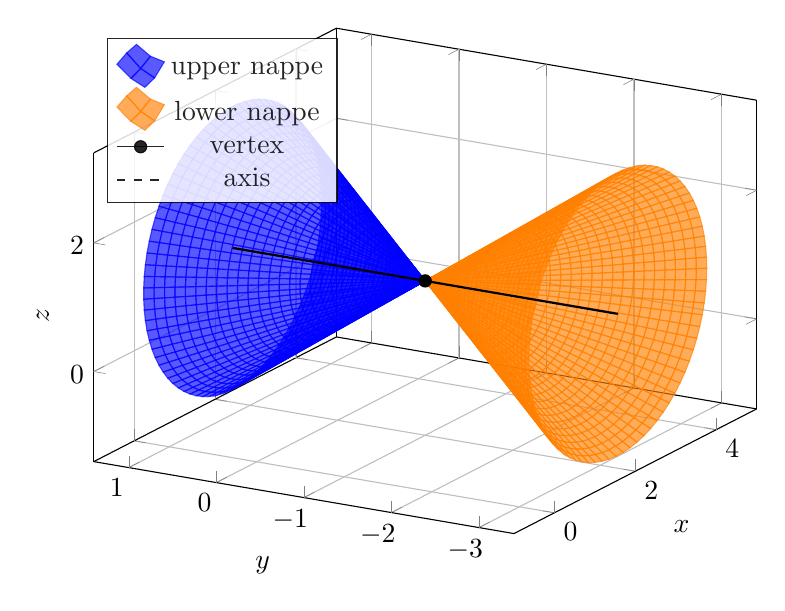
\begin{tikzpicture}
\begin{axis}[
  width=10cm,
  height=8cm,
  view={-60}{25},
  xlabel={$x$}, ylabel={$y$}, zlabel={$z$},
  domain=0:2.2,
  y domain=0:360,
  samples=28,
  samples y=80,
  grid=major,
  xmin=-1, xmax=5,
  ymin=-3.4, ymax=1.4,
  zmin=-1.4, zmax=3.4,
  legend style={at={(0.02,0.98)}, anchor=north west, fill=white, opacity=0.85}
]
\addplot3[surf, shader=flat, blue, opacity=0.65]
  ({2+x*cos(y)}, {-1+x}, {1+x*sin(y)});
\addlegendentry{upper nappe}
\addplot3[surf, shader=flat, orange, opacity=0.65]
  ({2+x*cos(y)}, {-1-x}, {1+x*sin(y)});
\addlegendentry{lower nappe}
\addplot3[black, mark=*, mark size=2.2pt] coordinates {(2,-1,1)};
\addlegendentry{vertex}
\addplot3[black, dashed, thick, domain=-2.2:2.2, samples=2]
  ({2}, {-1+x}, {1});
\addlegendentry{axis}
\end{axis}
\end{tikzpicture}
\end{document}
